\documentclass[11pt, oneside, numbers=noenddot]{scrbook}

\usepackage{style}

\def\Title{OSI 7 Schichtenmodell}	
\def\Subtitle{Layer 1}


\begin{document}


\titlehead{%
\begin{minipage}[c]{0.20\linewidth}

\includegraphics[width=0.8\linewidth]{htl_c_cmyk_rein.pdf}
\end{minipage}
\begin{minipage}[c]{0.5\linewidth}
\begin{center}
{\bfseries\sffamily\large Höhere  technische  Bundeslehranstalt\\
und  Bundesfachschule\\
{\normalsize im Hermann Fuchs Bundesschulzentrum} }
\end{center}
\end{minipage}
\begin{minipage}[c]{0.2\linewidth}
\hfill 
\includegraphics[width=0.8\linewidth]{htl-bildung-mit-zukunft.png}
\end{minipage}\\
}
\title{\vspace{4em}\Title}

\subtitle{\Subtitle}


\author{\\[2,5em] 
\emph{Erstellt von:} \\[0,5em]
Michel Rögl-Brunner, BEd
}
\date{\vspace{3\baselineskip}\small Letzte Änderung: \todayshort}

\begin{titlepage}	
\maketitle
\end{titlepage}
\IfFileExists{revisions.tex}{\clearpage\input{revisions.tex}}{}
\cleardoublepage
\pdfbookmark[1]{Inhaltsverzeichnis}{toc}
\tableofcontents
\clearpage
\pagenumbering{arabic}

\chapter{OSI-Modell und Layer 1}
\section{Grundlagen des OSI-Modells}
Das OSI-Modell beschreibt die Kommunikation in Netzwerken in sieben Schichten. Jede Schicht hat klar definierte Aufgaben und bietet der darueberliegenden Schicht einen Dienst.

\begin{longtable}{|c|l|p{8cm}|}
\hline
\textbf{Layer} & \textbf{Name} & \textbf{Kernaufgabe} \\
\hline
7 & Application & Schnittstelle zu Anwendungen (z.\,B. HTTP, DNS, SMTP). \\
\hline
6 & Presentation & Datenformat, Kodierung, Kompression, Verschluesselung. \\
\hline
5 & Session & Aufbau, Steuerung und Abbau von Sitzungen. \\
\hline
4 & Transport & Ende-zu-Ende-Transport, Zuverlaessigkeit, Ports (TCP/UDP). \\
\hline
3 & Network & Logische Adressierung und Routing (IP). \\
\hline
2 & Data Link & Frames, MAC-Adressen, Fehlererkennung im lokalen Netz. \\
\hline
1 & Physical & Uebertragung von Bits als elektrische, optische oder Funk-Signale. \\
\hline
\end{longtable}

Diese Unterlage fokussiert auf \textbf{Layer 1}. Typische Themen dort sind:
\begin{itemize}
\item Uebertragungsmedien (Kupfer, Glasfaser, Funk)
\item Steckertypen und Pinbelegungen
\item Signalpegel, Daempfung, Stoerungen
\item Maximale Reichweiten und physikalische Grenzwerte
\end{itemize}

\section{Kabeltypen und Verbindungstypen auf Layer 1}
\subsection{Kupfer (Twisted Pair)}
Twisted-Pair-Kabel bestehen aus verdrillten Adernpaaren. Die Verdrillung reduziert elektromagnetische Einstreuungen und Nebensprechen (\textit{Crosstalk}), weil Stoersignale auf beide Leiter eines Paares aehnlich einwirken und sich differenziell besser unterdruecken lassen.

\begin{figure}[H]
\centering
\IfFileExists{Work/Aufgaben/OSI-Modell/Layer1/images/utp_cable.jpg}{%
  
\includegraphics[width=0.6\textwidth]{Work/Aufgaben/OSI-Modell/Layer1/images/utp_cable.jpg}%
}{%
  \IfFileExists{images/utp_cable.jpg}{%
    
\includegraphics[width=0.6\textwidth]{images/utp_cable.jpg}%
  }{%
    \fbox{\parbox{0.85\textwidth}{Bild fehlt: \texttt{images/utp\_cable.jpg}}}%
  }%
}
\caption{Beispiel eines UTP-Kabels (Quelle: Wikimedia Commons, Datei: UTP\_cable.jpg)}
\end{figure}

\subsubsection{UTP, STP, FTP, S/FTP}
Die Bezeichnungen geben an, ob ein Gesamtschirm und/oder ein Paarschirm vorhanden ist:
\begin{itemize}
\item \textbf{U/UTP (UTP):} Kein Gesamtschirm, kein Paarschirm. Guenstig, flexibel, in Buero-/Schulumgebungen haeufig.
\item \textbf{F/UTP (oft FTP genannt):} Folien-Gesamtschirm um alle Paare.
\item \textbf{S/UTP (oft STP genannt):} Geflecht-Gesamtschirm um alle Paare.
\item \textbf{S/FTP:} Geflecht-Gesamtschirm plus Folien-Schirm je Adernpaar. Sehr gute EMV-Eigenschaften.
\end{itemize}

Grundregel: Je staerker die Stoerquelle (z.\,B. Maschinen, Motoren, lange parallele Stromfuehrung), desto wichtiger ist eine gute Schirmung und saubere Erdung.

\subsubsection{Cat-Standards bei Kupferkabeln}
Die Kategorie (\textit{Category}, Cat) beschreibt die Uebertragungseigenschaften der Kupferverkabelung.

\begin{longtable}{|l|l|l|l|}
\hline
\textbf{Kategorie} & \textbf{Bandbreite} & \textbf{Typische Datenraten} & \textbf{Typische Verwendung} \\
\hline
Cat5e & 100 MHz & 1 Gbit/s bis 100 m & Standard-LAN, Schul-/Buero-Netz \\
\hline
Cat6 & 250 MHz & 1 Gbit/s bis 100 m, 10 Gbit/s bis ca. 55 m & Neuinstallationen mit Reserve \\
\hline
Cat6A & 500 MHz & 10 Gbit/s bis 100 m & Professionelle strukturierte Verkabelung \\
\hline
Cat8 & 2000 MHz & 25/40 Gbit/s bis 30 m & Rechenzentrum, kurze High-Speed-Links \\
\hline
\end{longtable}

Hinweis: Cat7/7A existieren als ISO/IEC-Klassen, sind aber im TIA-Umfeld nicht als klassische Cat-TIA-Stufen wie Cat6A/Cat8 verankert.

\subsubsection{Farbcode T568A und T568B}
Fuer RJ45 (8P8C) sind zwei Belegungsvarianten ueblich: T568A und T568B. Technisch sind beide gleichwertig, wichtig ist die \textbf{konsistente Nutzung} innerhalb einer Installation.

\begin{longtable}{|c|l|l|}
\hline
\textbf{Pin} & \textbf{T568A} & \textbf{T568B} \\
\hline
1 & Weiss/Gruen & Weiss/Orange \\
\hline
2 & Gruen & Orange \\
\hline
3 & Weiss/Orange & Weiss/Gruen \\
\hline
4 & Blau & Blau \\
\hline
5 & Weiss/Blau & Weiss/Blau \\
\hline
6 & Orange & Gruen \\
\hline
7 & Weiss/Braun & Weiss/Braun \\
\hline
8 & Braun & Braun \\
\hline
\end{longtable}

In der Praxis wird in vielen europaeischen Installationen haeufig T568B verwendet. Normativ sind beide Varianten zulaessig, solange nicht gemischt wird.

\subsubsection{Was ist ein Crossover-Kabel?}
Ein Crossover-Kabel ist an einem Ende nach T568A und am anderen Ende nach T568B aufgelegt. Dadurch werden Sende- und Empfangsadern gekreuzt. Frueher war das fuer direkte Verbindungen gleichartiger Geraete relevant (z.\,B. Switch zu Switch). Heute erkennen viele Geraete den Leitungstyp automatisch (\textit{Auto-MDI/X}).

\subsection{Glasfaser (LWL)}
LWL (Lichtwellenleiter) uebertraegt Daten als Lichtimpulse statt als elektrische Signale. Dadurch ist die Uebertragung unempfindlich gegen elektromagnetische Stoerungen.

\subsubsection{Singlemode vs. Multimode}
\begin{longtable}{|l|l|l|}
\hline
\textbf{Merkmal} & \textbf{Singlemode (OS1/OS2)} & \textbf{Multimode (OM1-OM5)} \\
\hline
Kerndurchmesser & ca. 9 um & 50 oder 62.5 um \\
\hline
Lichtquelle & Laser (typ. 1310/1550 nm) & LED/VCSEL (typ. 850/1300 nm) \\
\hline
Reichweite & Sehr hoch (km-Bereich) & Eher kurz bis mittel (typ. Gebaeude/DC) \\
\hline
Typischer Einsatz & Backbone, Campus, FTTH, WAN & Rechenzentrum, Inhouse-Verkabelung \\
\hline
\end{longtable}

\begin{figure}[H]
\centering
\IfFileExists{Work/Aufgaben/OSI-Modell/Layer1/images/multimode_vs_singlemode.png}{%
  
\includegraphics[width=0.75\textwidth]{Work/Aufgaben/OSI-Modell/Layer1/images/multimode_vs_singlemode.png}%
}{%
  \IfFileExists{images/multimode_vs_singlemode.png}{%
    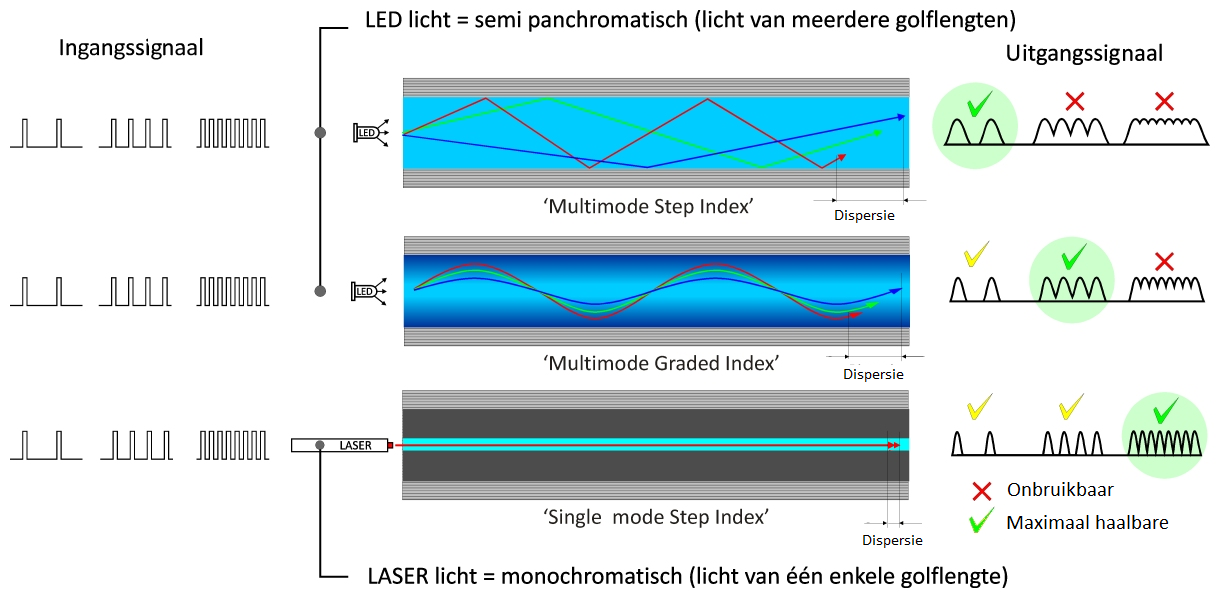
\includegraphics[width=0.75\textwidth]{images/multimode_vs_singlemode.png}%
  }{%
    \fbox{\parbox{0.85\textwidth}{Bild fehlt: \texttt{images/multimode\_vs\_singlemode.png}}}%
  }%
}
\caption{Singlemode vs. Multimode (Quelle: Wikimedia Commons, Datei: Multimode\_vs\_Single\_Mode\_Fiber.png)}
\end{figure}

\subsection{Funk (WLAN)}
WLAN basiert auf IEEE 802.11 und nutzt auf Layer 1 Funkwellen statt Kabel.
\begin{itemize}
\item \textbf{2.4 GHz:} Gute Reichweite und Durchdringung, aber stoeranfaelliger und meist geringere nutzbare Datenrate.
\item \textbf{5 GHz:} Hoehere Datenraten, mehr Kanaele, geringere Reichweite als 2.4 GHz.
\item \textbf{6 GHz (Wi-Fi 6E/7):} Sehr viele freie Kanaele, hohe Datenraten, kurze Reichweite und hohe Daempfung.
\end{itemize}

Bei WLAN gilt: Hoehere Frequenz bringt oft mehr Geschwindigkeit, aber meist weniger Reichweite pro Access Point.

\section{Vergleich Kupfer vs. Glasfaser (LWL)}
\begin{longtable}{|p{3.2cm}|p{5.3cm}|p{5.3cm}|}
\hline
\textbf{Kriterium} & \textbf{Kupfer (Twisted Pair)} & \textbf{Glasfaser (LWL)} \\
\hline
EMI-Stoeranfaelligkeit & Hoeher, je nach Schirmung besser beherrschbar & Sehr gering, da optische Uebertragung \\
\hline
Max. Reichweite pro Link & Typisch 100 m (LAN-Standard) & Von hunderten Metern bis viele Kilometer \\
\hline
Bandbreiten-Reserve & Hoch, aber physikalisch frueher limitiert & Sehr hoch, besonders fuer Backbone/Skalierung \\
\hline
Kosten der Aktivkomponenten & Oft guenstiger (Kupferports) & Optiken/Module oft teurer \\
\hline
Installation & Einfach, robust im Alltag, bekannte RJ45-Technik & Sorgfalt bei Reinigung, Biegeradius und Spleiss/Stecktechnik \\
\hline
Galvanische Trennung & Nicht gegeben & Gegeben, dadurch Vorteil bei Potenzialunterschieden \\
\hline
\end{longtable}

\subsection*{Wann nimmt man was?}
\begin{itemize}
\item \textbf{Kupfer (Twisted Pair):} Arbeitsplatzverkabelung, kurze bis mittlere Strecken in Gebaeuden, gutes Preis-Leistungs-Verhaeltnis.
\item \textbf{LWL:} Backbone zwischen Verteilern/Gebaeuden, lange Strecken, hohe Bandbreite und Umgebungen mit starker EMV-Belastung.
\end{itemize}

\section{Zusammenfassung}
Layer 1 bildet die technische Basis jeder Netzkommunikation. Die Wahl des Mediums entscheidet direkt ueber Reichweite, Stabilitaet, Datenrate und Kosten:
\begin{itemize}
\item Kupfer ist fuer viele Standard-LAN-Szenarien wirtschaftlich und praxisnah.
\item LWL ist bei grossen Distanzen, hohen Bandbreiten und EMV-Anforderungen klar im Vorteil.
\item WLAN erweitert Layer 1 um Mobilitaet, benoetigt aber sorgfaeltige Funkplanung.
\end{itemize}

\section*{Quellen (Auswahl)}
\begin{itemize}
\item Fluke Networks: \texttt{https://www.flukenetworks.com/knowledge-base/application-or-standards-articles-copper/differences-between-wiring-codes-t568a-vs}
\item ANSI/TIA-568 Uebersicht: \texttt{https://en.wikipedia.org/wiki/ANSI/TIA-568}
\item Eaton/Tripp Lite Ethernet Cables: \texttt{https://tripplite.eaton.com/products/ethernet-cable-types}
\item Tektronix 802.11 PHY Primer: \texttt{https://www.tek.com/en/documents/primer/wi-fi-overview-80211-physical-layer-and-transmitter-measurements}
\item Twisted Pair Grundlagen: \texttt{https://en.wikipedia.org/wiki/Twisted_pair}
\item LWL Singlemode vs Multimode: \texttt{https://commons.wikimedia.org/wiki/File:Multimode_vs_Single_Mode_Fiber.png}
\end{itemize}

\end{document}